\chapter{MESONH grid}  \label{a:grid}

MESO-NH use a C-grid in the Arakawa convention, both on the horizontal and on the vertical.
This grid is shown on the following figure :
\begin{itemize}
\item 1 : mass points 
\item 2 : u  points
\item 3 : v  points
\item 4 : w  points
\item 5 : vertical vorticity point
\item 6 : vorticity components along y
\item 7 : vorticity components along x
\end{itemize}
\begin{center}
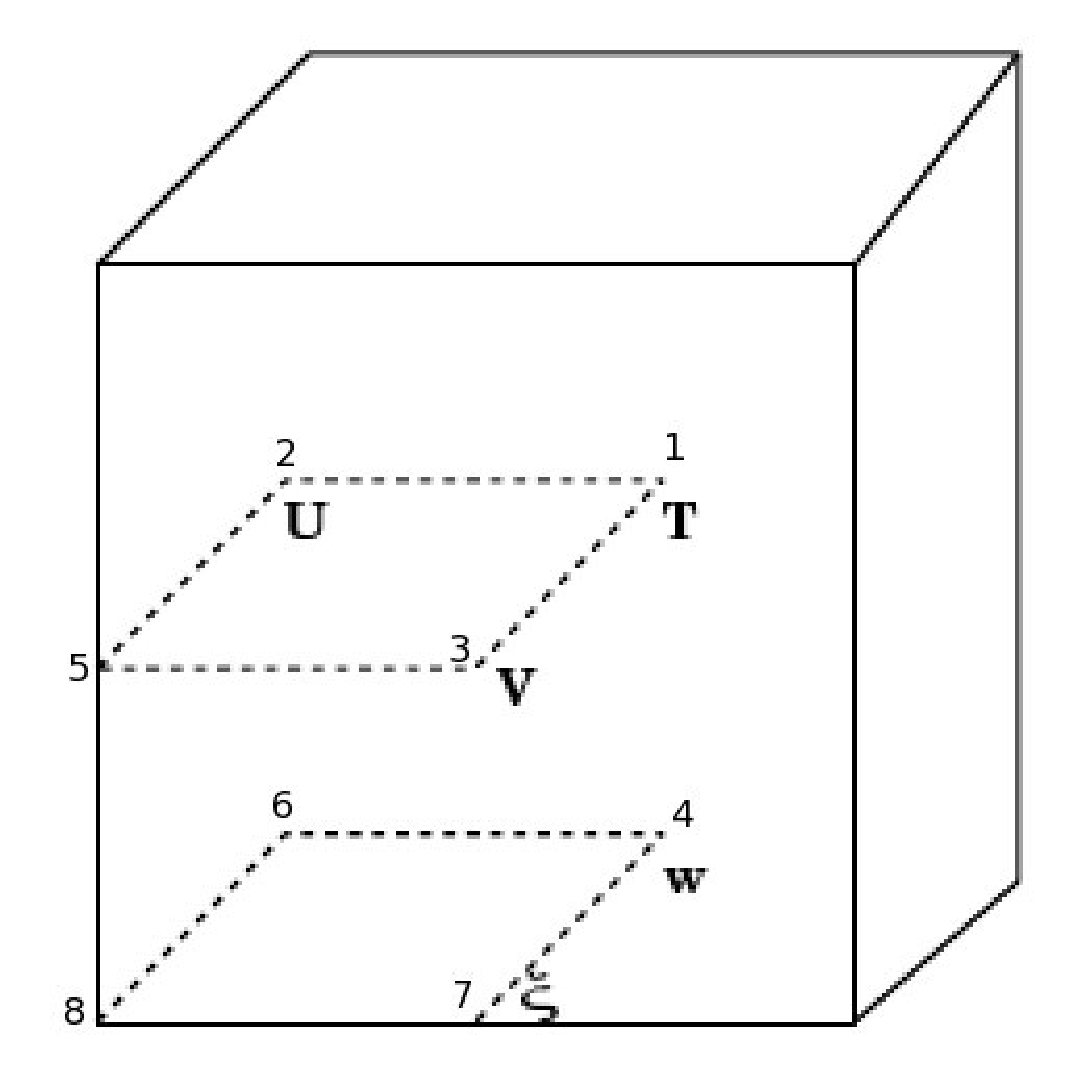
\includegraphics[width=8cm]{annexes/grilles}
\end{center}
